\documentclass[conference,a4paper,10pt]{IEEEtran}

\usepackage{fontspec}
\setmainfont{TeX Gyre Termes}
\usepackage{amsmath,amssymb,booktabs,graphicx,microtype,tabularx,array,url,xurl,xspace}
\usepackage{balance}
\usepackage[hidelinks]{hyperref}
\usepackage[backend=biber,style=numeric,sorting=none,maxbibnames=4,giveninits=true,doi=false,url=false,isbn=false]{biblatex}
\addbibresource{../src/bib/manual.bib}
\addbibresource{../src/bib/agent.bib}
\addbibresource{../src/bib/ingestion.bib}

\graphicspath{{../src/images/}{../src/images/manual/}{../src/images/experiments/customer_service_revision/final_eda/}{../src/images/experiments/legal_revision/final_eda/}}

\newcommand{\chunker}{\textit{chunker}\xspace}
\newcommand{\indexer}{\textit{indexer}\xspace}
\newcommand{\kg}{\textit{knowledge graph}\xspace}
\newcommand{\plugin}{\textit{plugin}\xspace}
\newcommand{\artifact}{\textit{artifact}\xspace}
\newcommand{\retrieval}{\textit{retrieval}\xspace}
\newcommand{\omnirag}{OMNI-RAG\xspace}
\newcommand{\code}[1]{\texttt{#1}}

\setlength{\emergencystretch}{2em}
\renewcommand{\arraystretch}{1.08}

\title{Konstruksi Basis Pengetahuan Modular pada OMNI-RAG Multi-Domain:\\
Evaluasi Chunker, Indexer, dan Legal Knowledge Graph}

\author{
\IEEEauthorblockN{Moh Fairuz Alauddin Yahya}
\IEEEauthorblockA{Program Studi Informatika\\
Institut Teknologi Bandung\\
Bandung, Indonesia\\
13522057@std.stei.itb.ac.id}
\and
\IEEEauthorblockN{Agung Dewandaru}
\IEEEauthorblockA{Institut Teknologi Bandung\\
Bandung, Indonesia\\
dewandaru@itb.ac.id}
\and
\IEEEauthorblockN{I Wayan Gunada}
\IEEEauthorblockA{Institut Teknologi Bandung\\
Bandung, Indonesia\\
gunada@itb.ac.id}}

\begin{document}
\maketitle

\begin{abstract}
Pipeline \textit{Retrieval-Augmented Generation} (RAG) harus mengubah dokumen yang beragam menjadi unit informasi yang dapat dicari sebelum model bahasa menyusun jawaban. Paper ini menyajikan pendekatan modular berbasis representasi kanonik dan antarmuka \plugin umum untuk konstruksi basis pengetahuan pada \omnirag. Fokus evaluasi bukan rincian mekanisme plugin, melainkan perbandingan strategi \chunker, \indexer, dan \kg ketika hanya satu komponen diubah. Eksperimen \textit{one factor at a time} menggunakan sembilan manual Netgear (1.400 halaman, 200 pertanyaan bilingual) dan korpus hukum (256 dokumen, 25 pertanyaan terverifikasi). Pada $K=30$, \textit{structure-aware hybrid} menghasilkan \textit{recall} 0,740 pada manual, sedangkan \textit{structure-aware dense} menghasilkan 0,785. Pada korpus hukum, \textit{legal-structure dense} menghasilkan 0,6854 dan hybrid memiliki MRR tertinggi, 0,5439. Traversal graf hingga kedalaman dua mencapai \textit{neighborhood recall} 1,0000 pada konfigurasi \textit{sliding}. Hasil menunjukkan bahwa pemeliharaan struktur dan pencocokan semantik meningkatkan cakupan konteks, tetapi konfigurasi terbaik bergantung pada domain serta metrik yang diprioritaskan.
\end{abstract}

\begin{IEEEkeywords}
OMNI-RAG, basis pengetahuan, chunking, indexing, knowledge graph, plugin, retrieval augmented generation.
\end{IEEEkeywords}

\section{Pendahuluan}

Sistem tanya jawab berbasis \textit{large language model} (LLM) membutuhkan sumber eksternal agar jawaban tidak hanya bergantung pada pengetahuan parametrik model. \textit{Retrieval-Augmented Generation} (RAG) menyediakan sumber tersebut dengan mengambil potongan dokumen sebelum proses generasi \cite{lewisRetrievalAugmentedGenerationKnowledgeIntensive2021,huangSurveyRetrievalAugmentedText2024}. Tantangannya bukan sekadar menyimpan dokumen. Dokumen hukum memiliki hierarki Bab, Bagian, Pasal, Ayat, Huruf, dan Angka, sedangkan \textit{User Manual} berisi struktur yang lebih bebas seperti heading, langkah prosedural, tabel, dan peringatan. Jika batas potongan, representasi indeks, atau hubungan antardokumen dibentuk tanpa memperhatikan struktur, konteks yang dibutuhkan dapat terpisah atau sulit ditemukan.

Paper ini mengambil satu kontribusi teknis dari platform \omnirag yang dikembangkan dalam proyek Capstone empat orang. Konteks tersebut hanya diperlukan untuk menempatkan jalur konstruksi basis pengetahuan di antara komponen sistem lain; pembahasan dan evaluasi di sini dibatasi pada pekerjaan individu penulis. Jalur yang dipelajari adalah pemrosesan \textit{offline} dari dokumen kanonik menjadi potongan, indeks, dan graf yang dapat dipakai oleh tahap \retrieval.

Tiga masalah penelitian dirumuskan sebagai berikut.

\begin{enumerate}
    \item Bagaimana strategi \chunker dapat membentuk unit informasi yang mempertahankan konteks struktural pada dokumen dengan karakteristik berbeda?
    \item Bagaimana strategi \indexer sparse, dense, dan hybrid memengaruhi kelengkapan serta urutan konteks yang ditemukan?
    \item Bagaimana \kg dibangun dari unit yang sama dan digunakan untuk memperluas jangkauan dokumen tanpa mengaburkan provenance sumber?
\end{enumerate}

Kontribusi paper ini adalah (1) rancangan kontrak artefak kanonik yang menghubungkan parser, \chunker, \indexer, dan \kg; (2) implementasi arsitektur \plugin dan \profile yang memungkinkan strategi diganti tanpa mengubah orkestrator; (3) legal \kg deterministik yang merepresentasikan hubungan perubahan peraturan; dan (4) evaluasi terkontrol pada korpus manual produk dan peraturan pendidikan Indonesia. Evaluasi tidak menggabungkan hasil lintas konfigurasi: setiap konfigurasi memakai korpus, pertanyaan, parser, dan model embedding yang sama ketika satu faktor sedang dibandingkan.

Ruang lingkup paper adalah konstruksi basis pengetahuan dan dampaknya pada \retrieval serta generation. Tahap akuisisi dan parsing diperlakukan sebagai pemasok dokumen kanonik, sedangkan komponen percakapan berada di luar klaim penelitian ini. Dengan batas tersebut, bagian berikutnya membahas landasan teknis, rancangan pipeline, metode eksperimen, hasil, dan implikasinya.

\section{Landasan dan Posisi Penelitian}

\subsection{Unit Dokumen dan Chunking}

\textit{Chunking} menentukan unit yang akan disimpan, dicari, dan diberikan kepada generator. Potongan terlalu besar membawa noise dan melampaui anggaran konteks, sedangkan potongan terlalu kecil dapat memisahkan definisi, syarat, pengecualian, atau hubungan antarbagian. Studi NitiBench menunjukkan bahwa pemotongan berbasis struktur dapat memberikan hasil berbeda dari strategi generik pada pertanyaan hukum \cite{akarajaradwongNitiBenchComprehensiveStudy2025}. Karena itu, batas potongan diperlakukan sebagai keputusan desain yang perlu diuji pada domain target, bukan sebagai parameter universal.

Penelitian ini membandingkan \textit{sliding-window}, \textit{recursive}, \textit{generic structure-aware}, dan \textit{legal structure-aware}. Strategi generik memanfaatkan outline parser dan dapat membawa konteks heading induk. Strategi legal memusatkan unit pada Pasal, mempertahankan konteks Bab atau Bagian, lalu dapat membentuk \textit{child chunk} sebagai kandidat dan \textit{parent chunk} sebagai konteks lengkap.

\subsection{Indexer dan Representasi Pencarian}

Indexer leksikal seperti BM25 memberi bobot pada istilah yang jarang dan menormalisasi panjang dokumen \cite{robertsonProbabilisticRelevanceFramework2009}. Dense retrieval memetakan kueri dan unit teks menjadi vektor sehingga parafrasa dapat ditemukan meskipun tidak memiliki kata yang sama \cite{karpukhinDensePassageRetrieval2020}. BAAI/BGE-M3 dipakai sebagai model embedding multibahasa untuk eksperimen ini \cite{chenM3Embedding2024}. Hybrid retrieval menggabungkan daftar leksikal dan dense melalui Reciprocal Rank Fusion \cite{cormackReciprocalRankFusion2009}.

Perbedaan ketiga representasi penting pada dokumen hukum. Nomor peraturan dan nomor Pasal membutuhkan kecocokan literal, sementara pertanyaan pengguna dapat memparafrasekan norma. Skor dense dipahami sebagai kedekatan representasi, bukan putusan bahwa dua teks memiliki makna hukum yang identik. Identitas dokumen, struktur, metadata, dan provenance tetap menjadi dasar yang dapat diperiksa.

\subsection{Knowledge Graph sebagai Proyeksi Pelengkap}

\kg merepresentasikan entitas dan hubungan sebagai graf $G=(V,E)$ dengan sisi bertipe. Graf dapat menampung hubungan eksplisit yang tidak selalu muncul sebagai kemiripan teks, misalnya peraturan yang mengubah, menetapkan, atau mencabut peraturan lain. Paper ini membedakan dukungan graf opsional dari \textit{GraphRAG}: indeks teks tetap menghasilkan seed, lalu graf memperluas lingkungan dokumen seed; graf bukan pengganti pencarian teks atau mekanisme ringkasan komunitas utama \cite{edgeFromLocalGlobalGraph2024,hanRetrievalAugmentedGenerationGraphs2025}.

Desain modular diperlukan karena strategi yang baik pada satu domain belum tentu baik pada domain lain. Modular RAG memisahkan komponen yang dapat diganti, sedangkan kontrak antarmuka menjaga agar perubahan strategi tidak menyebar ke orkestrator \cite{gaoModularRAG2024,garlanIntroductionSoftware1994}. Penelitian ini menerapkan prinsip tersebut pada artefak pengetahuan dan mengujinya melalui hasil retrieval yang terukur.

\section{Rancangan Pipeline Konstruksi Basis Pengetahuan}

\subsection{Pendekatan Modular}

Paper ini memandang \plugin sebagai unit penggantian strategi, bukan sebagai topik implementasi tersendiri. Orkestrator hanya mengatur urutan tahap dan membaca artefak dengan tipe yang sama; keputusan tentang cara membentuk chunk, indeks, atau graf ditempatkan pada komponen yang dipilih. Dengan batas tersebut, perbandingan antarkomponen dapat dilakukan tanpa mengubah tahap hilir secara bersamaan.

Satu dokumen hasil parser menjadi sumber bersama untuk tiga proyeksi: unit pencarian melalui \chunker, representasi pencarian melalui \indexer, dan hubungan antardokumen melalui \kg. Representasi kanonik menjadi titik temu ketiganya. Provenance dan metadata dipertahankan sebagai bagian dari artefak sehingga hasil tiap strategi dapat ditelusuri kembali ke dokumen serta konfigurasi asalnya.

\begin{table}[t]
\centering
\caption{Peran artefak pada pendekatan modular}
\label{tab:kontrak-artefak}
\scriptsize
\begin{tabularx}{\columnwidth}{@{}p{0.31\columnwidth}X@{}}
\toprule
\textbf{Artefak} & \textbf{Peran dalam perbandingan}\\
\midrule
\code{CanonicalDocument} & Dokumen terurai yang memuat teks, hierarki, lokasi sumber, dan metadata; menjadi masukan semua strategi \chunker.\\
\code{CanonicalChunks} & Unit retrieval dan context dengan identitas posisi serta provenance; dipakai bersama oleh \indexer dan \kg.\\
\code{CanonicalIndex} & Proyeksi lexical, dense, atau hybrid dari chunk; menjadi masukan jalur direct retrieval.\\
\code{CanonicalGraph} & Proyeksi simpul dan relasi beserta bukti sumber; dipakai opsional untuk memperluas lingkungan dokumen.\\
\bottomrule
\end{tabularx}
\end{table}

Kontrak antarmuka menjaga agar keluaran setiap strategi dapat dikonsumsi tahap berikutnya dengan bentuk yang konsisten. Pemilihan strategi dilakukan melalui konfigurasi pipeline, sedangkan provenance mencatat komponen, versi, dan artefak yang digunakan. Dengan demikian, manfaat \plugin yang diuji dalam paper ini adalah keterpisahan faktor eksperimen: perubahan satu strategi tidak perlu disertai perubahan pada orkestrator atau format data downstream.

\subsection{Komponen yang Dibandingkan}

Kelompok \chunker membandingkan \textit{sliding-window}, \textit{recursive}, \textit{generic structure-aware}, dan \textit{legal structure-aware}. \textit{Sliding-window} menjadi baseline berbasis jendela tetap; \textit{recursive} memanfaatkan pemisah teks bertingkat; strategi structure-aware membawa heading atau hierarki hukum sebagai konteks. Pada dokumen hukum, parent chunk menjaga unit Pasal yang utuh sedangkan child chunk menjadi kandidat pencarian ketika unit tersebut terlalu panjang.

Kelompok \indexer membandingkan representasi sparse, dense, dan hybrid dari \code{CanonicalChunks}. Sparse mengandalkan kecocokan lexical, dense menggunakan embedding BAAI/BGE-M3, dan hybrid menggabungkan dua daftar kandidat dengan Reciprocal Rank Fusion. Perbedaan yang dibaca pada hasil adalah perbedaan representasi dan urutan kandidat, bukan perbedaan dokumen masukan.

Kelompok \kg menggunakan legal graph deterministik sebagai proyeksi opsional. Graf memuat hubungan struktur dan perubahan peraturan, lalu menerima seed dari hasil top-$K$ retrieval. Traversal dibatasi oleh kedalaman, arah, jenis relasi, dan cakupan eksperimen; hasilnya dipetakan kembali ke chunk atau dokumen yang memiliki provenance. Karena itu, graf memperluas lingkungan dokumen tanpa menggantikan text retrieval sebagai sumber bukti utama.

\subsection{Cara Pendekatan Diuji}

Setiap kelompok membandingkan satu faktor pada satu waktu. Ketika \chunker diuji, datasource, parser, embedding, dan \indexer dikunci. Ketika \indexer diuji, \chunker dan seluruh input dikunci. Ketika \kg diuji, seed retrieval serta aturan traversal ditetapkan sebelum pengukuran. Direct retrieval mematikan reranker dan graf agar metrik retrieval tidak tercampur dengan tahap hilir.

Tiga klaim operasional kemudian diuji: (1) pemeliharaan struktur meningkatkan cakupan context reference dibandingkan fixed-window; (2) dense retrieval meningkatkan recall ketika kueri memparafrasekan istilah sumber, sementara hybrid dapat menguntungkan posisi hit pertama; dan (3) traversal legal graph memperluas jangkauan dokumen tetangga, tetapi neighborhood recall harus dibaca terpisah dari context-reference recall. Hasil tiap konfigurasi dilaporkan pada cutoff dan korpus yang sama sehingga perbedaan dapat dikaitkan dengan strategi yang dibandingkan.

\section{Metode Eksperimen}

\subsection{Lingkungan dan Korpus}

Pipeline dijalankan dengan Python 3.13 dengan lingkungan eksekusi, parser, dan model embedding BAAI/BGE-M3 pada CPU yang sama untuk seluruh run. Infrastruktur dan jumlah kandidat juga dikunci pada setiap perbandingan komponen sehingga perubahan skor dibaca sebagai dampak strategi yang diuji, bukan perubahan lingkungan.

\begin{table}[t]
\centering
\caption{Korpus dan unit evaluasi}
\label{tab:korpus}
\scriptsize
\begin{tabularx}{\columnwidth}{@{}p{0.25\columnwidth}X@{}}
\toprule
\textbf{Korpus} & \textbf{Cakupan dan acuan}\\
\midrule
\textit{User Manual} & 9 manual Netgear, 1.400 halaman, 100 slot bilingual, 200 pertanyaan, satu context reference per slot.\\
Peraturan pendidikan & 256 dokumen (49 memuat reference dan 207 noise), 25 pertanyaan terverifikasi, 148 baris reference, 144 context unik, 45 dokumen seed.\\
\bottomrule
\end{tabularx}
\end{table}

Pada corpus manual, sembilan dokumen meliputi CM2000, LM1200, R6350, R7000, RAX120, RAX50, RAXE500, RBK852, dan XR500. Pertanyaan dibentuk dari slot yang disampling terstratifikasi menurut dokumen dan posisi halaman, kemudian setiap slot diberi varian Inggris dan Indonesia. Pada corpus hukum, 49 dokumen yang memuat reference dipertahankan sebagai inti; 207 noise dipilih secara stratified berdasarkan kelompok bentuk, status, rentang tahun, dan panjang sehingga semua konfigurasi melihat datasource 256 dokumen yang sama.

\subsection{Protokol Perbandingan}

Eksperimen memakai \textit{one factor at a time} (OFAT) sebagai pendekatan utama. Pada kelompok chunker, datasource, parser, embedding, dan indexer dikunci; hanya strategi segmentasi yang berubah. Pada kelompok indexer, chunker dan seluruh input dikunci; hanya representasi lexical, dense, atau hybrid yang berubah. Pada kelompok graf, seed retrieval dan aturan traversal dikunci; hanya hasil perluasan lingkungan yang dibaca. Dengan demikian, antarmuka plugin menjadi alat pengendalian eksperimen: komponen dapat diganti, tetapi masukan dan keluaran yang dibandingkan tetap memiliki bentuk yang sama.

Jalur direct retrieval mematikan reranker dan \kg agar metrik retrieval tidak tercampur dengan tahap hilir. Sweep cutoff menggunakan $K=5,10,\ldots,60$; $K=30$ dipilih sebagai cutoff kandidat bersama untuk membaca trade-off coverage dan beban downstream. Generation menggunakan sepuluh evidence teratas ($K=10$).

Pertanyaan manual dihitung gabungan serta terpisah menurut bahasa. Pertanyaan hukum mencakup pendirian dan status institusi, kewenangan, akses mahasiswa, kualifikasi staf, penjaminan mutu, serta kepatuhan. Semua hasil dicatat per konfigurasi; hasil kandidat dari konfigurasi berbeda tidak digabungkan.

\subsection{Metrik}

Misalkan $G_q$ adalah himpunan context reference acuan untuk pertanyaan $q$, sedangkan $R_q(K)$ adalah himpunan chunk unik yang dikembalikan sampai cutoff $K$. Recall dan precision dihitung sebagai
\begin{equation}
\begin{aligned}
\operatorname{Recall}@K&=\frac{1}{|Q|}\sum_{q\in Q}\frac{|G_q\cap R_q(K)|}{|G_q|},\\
\operatorname{Precision}@K&=\frac{1}{|Q|}\sum_{q\in Q}\frac{|G_q\cap R_q(K)|}{K}.
\end{aligned}
\label{eq:recall-precision}
\end{equation}

MRR menilai posisi reference pertama. Jika $r_q$ adalah posisi tersebut, kontribusinya $1/r_q$ dan bernilai nol ketika reference tidak ditemukan. NDCG menggunakan label relevansi bertingkat 0, 1, dan 2 untuk membedakan konteks yang tidak mendukung, mendukung sebagian, dan mendukung langsung. Pada generation, \textit{correctness} mengukur kelengkapan jawaban terhadap acuan, sedangkan \textit{faithfulness} memeriksa dukungan klaim oleh evidence.

Untuk graf, reference dipetakan ke dokumen sumber. $N_q$ adalah himpunan dokumen tetangga acuan dan $H_q(K)$ adalah hasil setelah seed retrieval dan traversal global hingga kedalaman dua. Neighborhood recall didefinisikan sebagai
\begin{equation}
\operatorname{KGRecall}@K=\frac{1}{|Q|}\sum_{q\in Q}\frac{|N_q\cap H_q(K)|}{|N_q|}.
\label{eq:kg-recall}
\end{equation}

Metrik ini mengukur jangkauan lingkungan, bukan keberhasilan menemukan setiap context reference secara langsung. Oleh sebab itu, nilai graf dilaporkan terpisah dari Recall@K retrieval.

\subsection{Konfigurasi yang Dibandingkan}

\begin{table*}[t]
\centering
\caption{Konfigurasi OFAT pada dua korpus}
\label{tab:konfigurasi}
\scriptsize
\begin{tabularx}{\textwidth}{@{}p{0.18\textwidth}p{0.31\textwidth}X@{}}
\toprule
\textbf{Korpus dan kelompok} & \textbf{Level yang dibandingkan} & \textbf{Parameter tetap}\\
\midrule
Manual--chunker & structure-aware hybrid; recursive; sliding-window & 512 karakter, overlap 51 untuk recursive/sliding, hybrid indexer, parser dan embedding yang sama.\\
Manual--indexer & structure-aware dense; hybrid; structure-aware sparse & structure-aware chunker, BAAI/BGE-M3 untuk dense, lexical field dan corpus yang sama.\\
Hukum--chunker & legal-structure dense; recursive; sliding & parent hydration, 512 karakter untuk struktur legal, overlap 51 untuk recursive/sliding, dense indexer.\\
Hukum--indexer & legal-structure dense; structure-aware hybrid; structure-aware sparse & legal structure-aware chunker, corpus dan context reference yang sama; hybrid memakai RRF.\\
\bottomrule
\end{tabularx}
\end{table*}

Konfigurasi manual menggunakan satu context reference per slot sehingga perubahan Recall@K dapat dibaca langsung sebagai perubahan cakupan unit acuan. Konfigurasi hukum menggunakan 144 context reference unik; hubungan legal graph dibangun dari 17 relasi berarah dan 24 relasi tak berarah yang tersedia pada benchmark. Pemilihan $K=30$ tidak menyatakan bahwa seluruh kurva telah datar, melainkan menyediakan titik kerja yang sama untuk membandingkan komponen dan meneruskan kandidat ke tahap berikutnya.

\section{Hasil dan Pembahasan}

Hasil berikut dibaca sebagai perbandingan terkontrol, bukan sebagai satu peringkat universal untuk semua strategi. Dalam setiap kelompok, artefak masukan dan tahap hilir dipertahankan; hanya strategi yang menjadi faktor uji yang berubah. Recall mengukur kelengkapan context reference, sedangkan MRR dan NDCG menangkap perbedaan posisi serta kualitas ranking. Cara baca ini penting karena tujuan pipeline adalah memilih komponen sesuai domain dan tujuan tahap, bukan mencari satu plugin yang selalu terbaik.

\subsection{Hasil pada User Manual}

\begin{table}[t]
\centering
\caption{Hasil kelompok chunker pada User Manual, $K=30$}
\label{tab:hasil-manual-chunker}
\scriptsize
\begin{tabularx}{\columnwidth}{@{}p{0.37\columnwidth}rrrr@{}}
\toprule
\textbf{Strategi} & \textbf{R} & \textbf{P} & \textbf{N} & \textbf{M}\\
\midrule
Structure-aware hybrid & \textbf{0,740} & \textbf{0,048} & \textbf{0,333} & 0,231\\
Recursive & 0,625 & 0,032 & 0,291 & 0,216\\
Sliding-window & 0,685 & 0,041 & 0,322 & \textbf{0,232}\\
\bottomrule
\multicolumn{5}{l}{\scriptsize R: Recall, P: Precision, N: NDCG, M: MRR.}
\end{tabularx}
\end{table}

Pada kelompok chunker, structure-aware hybrid menghasilkan Recall@30 sebesar 0,740, lebih tinggi 0,055 daripada sliding-window dan 0,115 daripada recursive (Tabel~\ref{tab:hasil-manual-chunker}). Keunggulan tersebut juga muncul pada precision dan NDCG. Sliding-window memiliki MRR sedikit lebih tinggi, 0,232 berbanding 0,231, sehingga pemeliharaan struktur meningkatkan jumlah reference yang ditemukan tanpa selalu menempatkan reference pertama pada posisi paling awal. Ketika cutoff dinaikkan ke 60, recall hanya berubah menjadi 0,745, 0,685, dan 0,630; sebagian besar coverage tambahan sudah diperoleh sebelum ekor ranking.

\begin{table}[t]
\centering
\caption{Hasil kelompok indexer pada User Manual, $K=30$}
\label{tab:hasil-manual-indexer}
\scriptsize
\begin{tabularx}{\columnwidth}{@{}p{0.37\columnwidth}rrrr@{}}
\toprule
\textbf{Strategi} & \textbf{R} & \textbf{P} & \textbf{N} & \textbf{M}\\
\midrule
Structure-aware dense & \textbf{0,785} & \textbf{0,057} & \textbf{0,350} & \textbf{0,314}\\
Hybrid & 0,740 & 0,048 & 0,333 & 0,231\\
Structure-aware sparse & 0,420 & 0,028 & 0,157 & 0,120\\
\bottomrule
\multicolumn{5}{l}{\scriptsize R: Recall, P: Precision, N: NDCG, M: MRR.}
\end{tabularx}
\end{table}

Dense indexer memberikan hasil terbaik pada semua metrik retrieval manual (Tabel~\ref{tab:hasil-manual-indexer}). Selisih recall dense terhadap sparse adalah 0,365, sedangkan terhadap hybrid adalah 0,045. Pada $K=30$, recall dense untuk pertanyaan Inggris dan Indonesia masing-masing 0,810 dan 0,760; gap lintas bahasa 0,050 lebih kecil daripada hybrid (0,120) dan sparse (0,240). Hal ini konsisten dengan tujuan BGE-M3 untuk menemukan parafrasa multibahasa, tetapi tidak mengubah batasan bahwa kecocokan vektor bukan kesetaraan makna hukum.

\begin{figure}[t]
\centering

\includegraphics[width=\columnwidth]{metrics-at-sweet-spot-indexer.png}
\caption{Metrik indexer User Manual pada $K=30$.}
\label{fig:hasil-manual-indexer}
\end{figure}

Pada generation dengan $K=10$, dense menghasilkan correctness/faithfulness 0,788/0,958, hybrid 0,711/0,946, dan sparse 0,508/0,881. Payload dense justru paling kecil, sekitar 3.399 token, dibandingkan hybrid 3.514 dan sparse 3.708. Jadi peningkatan correctness tidak dijelaskan oleh jumlah token semata, melainkan oleh reference yang lebih lengkap dan lebih awal pada sepuluh evidence teratas.

\subsection{Hasil pada Peraturan Pendidikan}

\begin{table*}[t]
\centering
\caption{Hasil retrieval pada corpus hukum, $K=30$}
\label{tab:hasil-legal}
\scriptsize
\begin{tabularx}{\textwidth}{@{}p{0.31\textwidth}rrrr@{}}
\toprule
\textbf{Konfigurasi} & \textbf{Recall} & \textbf{Precision} & \textbf{NDCG} & \textbf{MRR}\\
\midrule
Legal-structure dense (kelompok chunker) & \textbf{0,6854} & \textbf{0,1520} & 0,5040 & \textbf{0,5240}\\
Recursive (kelompok chunker) & 0,6730 & 0,1453 & 0,4909 & 0,4937\\
Sliding (kelompok chunker) & 0,6345 & 0,1507 & \textbf{0,5042} & 0,4626\\
Structure-aware dense (kelompok indexer) & \textbf{0,6854} & \textbf{0,1520} & \textbf{0,5040} & 0,5240\\
Structure-aware sparse & 0,6381 & 0,1253 & 0,4262 & 0,4613\\
Structure-aware hybrid & 0,6412 & 0,1307 & 0,4797 & \textbf{0,5439}\\
\bottomrule
\end{tabularx}
\end{table*}

Legal-structure dense mengalahkan sliding baseline pada recall sebesar 0,0509 (Tabel~\ref{tab:hasil-legal}). Keunggulan tersebut berasal dari child chunk yang tetap membawa identitas Pasal dan konteks induk, bukan dari penambahan jumlah kandidat. Recursive berada dekat dengan dense karena kalimat yang bersebelahan sering tetap bersama; sliding hampir menyamai dense pada NDCG (0,5042 berbanding 0,5040), tetapi tidak menemukan sebanyak reference secara total.

Pada kelompok indexer, dense memperoleh recall 0,6854, sparse 0,6381, dan hybrid 0,6412. Hybrid memiliki MRR tertinggi, 0,5439, yang berarti satu reference pertama lebih sering muncul di posisi awal. Namun, tujuan utama pipeline adalah menyediakan sebanyak mungkin context reference untuk tahap berikutnya, sehingga dense tetap dipilih sebagai konfigurasi coverage. Perbedaan ini memperlihatkan bahwa recall dan posisi hit pertama mengukur sifat ranking yang berbeda.

\begin{figure}[t]
\centering

\includegraphics[width=\columnwidth]{metrics-at-sweet-spot.png}
\caption{Metrik seluruh konfigurasi hukum pada $K=30$.}
\label{fig:hasil-legal}
\end{figure}

Generation hukum memperkuat pola tersebut. Legal-structure dense menghasilkan correctness 0,690 dan faithfulness 0,972. Sparse menghasilkan 0,578/0,982, sedangkan hybrid menghasilkan 0,664/0,982. Faithfulness yang tinggi tidak berarti jawaban lengkap: evidence dapat mendukung klaim yang ditulis, tetapi tidak memuat seluruh rincian reference. Payload rata-rata ketiga indexer hampir sama, sehingga selisih correctness lebih tepat dibaca sebagai dampak coverage dan urutan evidence.

\subsection{Perluasan dengan Legal Knowledge Graph}

Eksperimen graf memetakan reference ke dokumen sumber, mengambil seed dari top-30 retrieval, lalu menelusuri neighborhood global sampai kedalaman dua. Pada benchmark hukum, graf memiliki 17 relasi berarah dan 24 relasi tak berarah. Neighborhood recall pada $K=30$ adalah 0,9556 untuk dense, 0,9975 untuk recursive, 1,0000 untuk sliding, 0,9672 untuk sparse, dan 0,9975 untuk hybrid.

\begin{figure}[t]
\centering
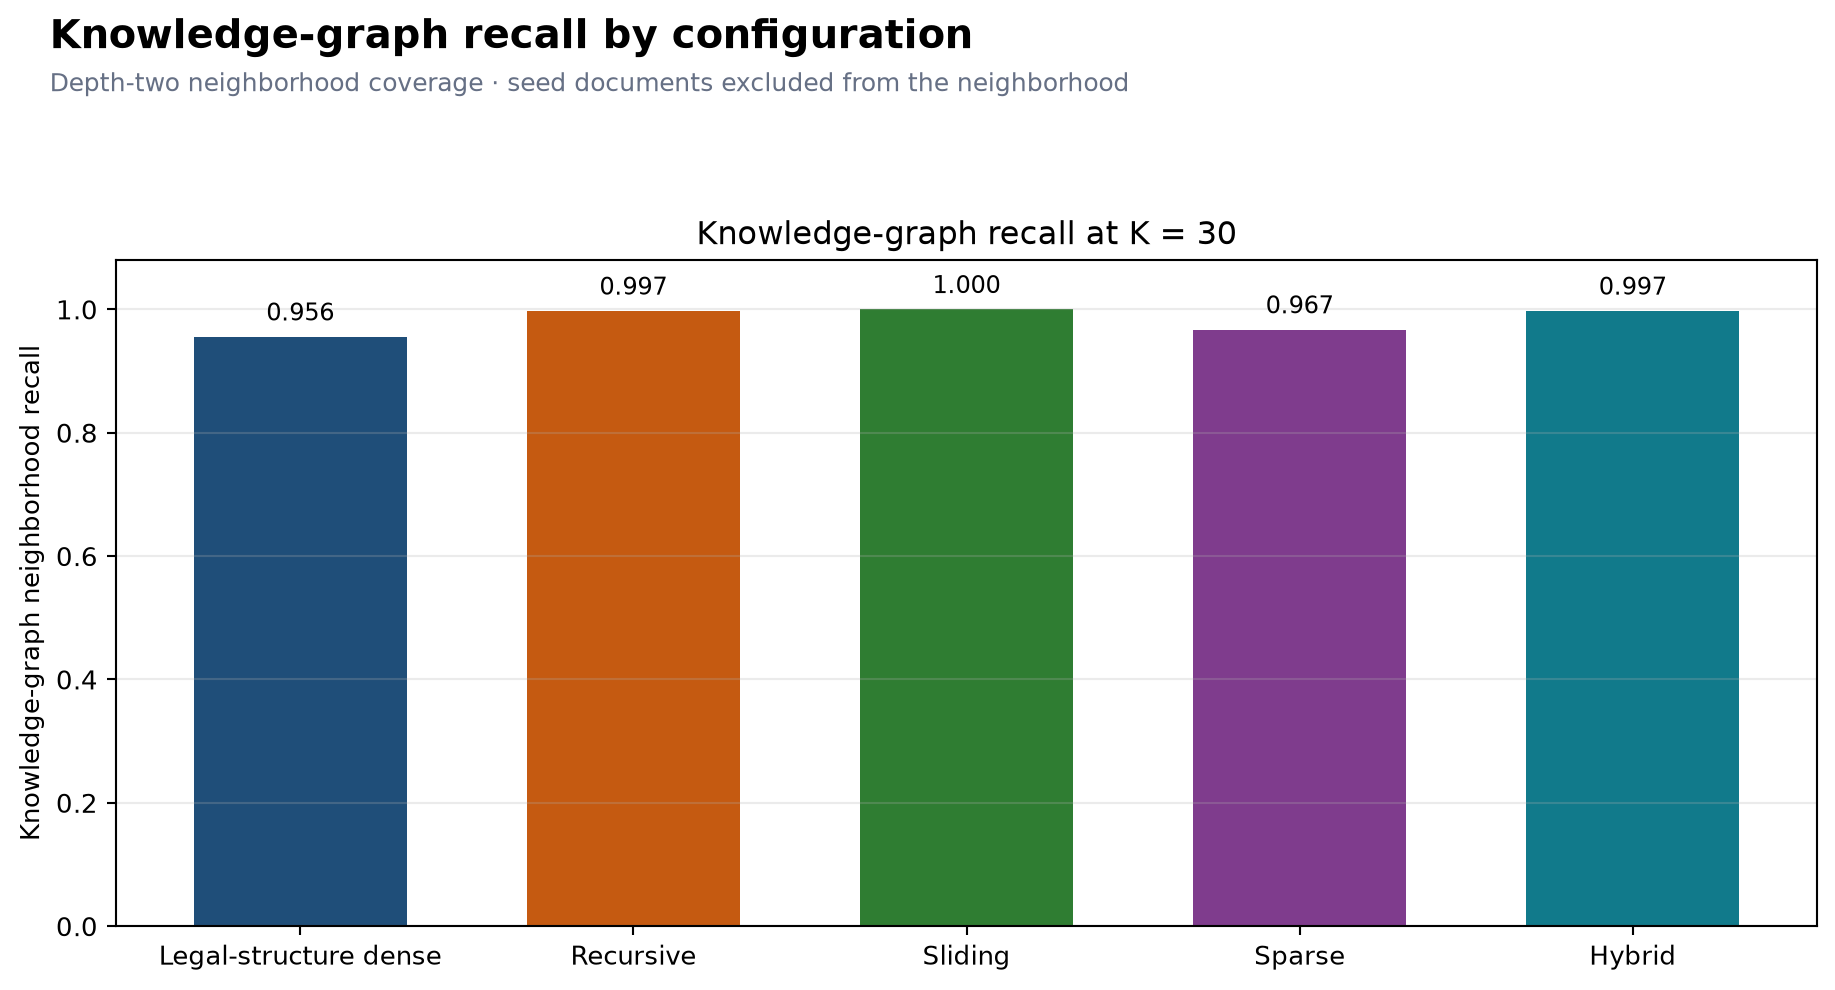
\includegraphics[width=\columnwidth]{kg-expanded-full-recall-k30.png}
\caption{Neighborhood recall legal graph pada $K=30$.}
\label{fig:hasil-kg}
\end{figure}

Nilai 1,0000 pada sliding tidak bertentangan dengan recall context reference yang lebih rendah. Satu dokumen seed dapat membuka beberapa dokumen tetangga melalui relasi perubahan, sehingga graf mengukur jangkauan lingkungan dan bukan ketepatan langsung setiap unit bukti. Temuan ini mendukung penggunaan graf sebagai proyeksi pelengkap: text retrieval memilih seed, sementara traversal menyediakan konteks lintas-dokumen yang eksplisit dan dapat ditelusuri.

\subsection{Pembahasan dan Keterbatasan}

Hasil dua korpus menunjukkan pola yang konsisten tetapi tidak identik. Structure-aware membantu ketika struktur sumber membawa informasi semantik, terutama pada legal-structure yang mempertahankan identitas Pasal dan parent context. Dense retrieval paling baik untuk coverage pada kedua domain, tetapi hybrid lebih baik untuk MRR hukum. Dengan demikian, tidak ada konfigurasi yang unggul pada seluruh metrik; tujuan tahap harus ditetapkan sebelum memilih komponen.

Pada level pendekatan, abstraksi plugin berfungsi sebagai pengendali eksperimen sekaligus batas rekayasa. Karena semua strategi menerima representasi kanonik dan mengembalikan proyeksi yang dikonsumsi tahap berikutnya, perbedaan pada tabel dapat dibahas sebagai perbedaan chunking, indexing, atau perluasan graf. Detail mekanisme pemuatan plugin tidak menjadi sumber temuan; nilai pendekatannya adalah memungkinkan perbandingan dan penggantian strategi tanpa menulis ulang jalur inti.

Kesimpulan ini bersifat kondisional pada corpus, pertanyaan, parser native-text, model BGE-M3, dan cutoff yang digunakan. Manual hanya mencakup sembilan produk Netgear dan 200 pertanyaan bilingual, sedangkan corpus hukum mencakup satu bidang dan 25 pertanyaan terverifikasi. OFAT tidak mengukur interaksi semua kombinasi parameter. Neighborhood recall juga tidak dapat dipakai sebagai pengganti context-reference recall. Perluasan corpus, anotasi relasi per pertanyaan, full factorial, dan pengujian model embedding hukum menjadi pekerjaan lanjutan yang wajar.

\section{Kesimpulan}

Paper ini menyajikan konstruksi basis pengetahuan modular untuk \omnirag multi-domain, dengan Capstone hanya sebagai konteks integrasi. Kontrak artefak kanonik membuat keluaran parser, \chunker, \indexer, dan \kg dapat dipertukarkan; \plugin Registry dan \profile memungkinkan strategi baru dipilih tanpa mengubah orkestrator. Dari empat strategi chunker, pemeliharaan struktur memberikan coverage lebih tinggi daripada fixed-window pada manual maupun peraturan. Dari tiga strategi indexer, dense BAAI/BGE-M3 memberikan Recall@30 tertinggi pada kedua corpus, sementara hybrid memiliki MRR hukum tertinggi. Legal graph deterministik memperluas seed retrieval ke neighborhood dokumen yang hampir atau sepenuhnya tercakup, tetapi metrik tersebut tetap dibaca terpisah dari recall context reference.

Secara empiris, konfigurasi utama adalah structure-aware dense untuk coverage manual (recall 0,785) dan legal-structure dense untuk coverage hukum (recall 0,6854). Hasil ini tidak menyatakan bahwa satu konfigurasi universal untuk semua domain; konfigurasi terbaik ditentukan oleh struktur dokumen dan tujuan metrik. Kontribusi utama penelitian adalah menunjukkan bagaimana keputusan tersebut dapat diuji secara terisolasi melalui kontrak, provenance, dan eksperimen OFAT.

Pengembangan berikutnya perlu memperluas corpus dan pertanyaan terverifikasi, menguji full factorial untuk interaksi chunker-indexer, melatih atau mengevaluasi embedding yang lebih spesifik untuk bahasa hukum Indonesia, serta mengukur kualitas relasi graf per jenis dan per pertanyaan. Artefak run dan provenance yang sudah disimpan menyediakan dasar untuk eksperimen tersebut.

\section*{Ucapan Terima Kasih}

Penulis berterima kasih kepada pembimbing dan anggota tim proyek yang menyediakan konteks integrasi sistem. Paper ini hanya menyajikan kontribusi penulis pada konstruksi basis pengetahuan dan tidak mengklaim kinerja komponen sistem di luar ruang lingkup tersebut.


\balance
\printbibliography[title={Daftar Pustaka}]
\end{document}
